\subsection{Émulation par interception}
\label{section:interception}
%% principe: interception des actions et médiation (pas juste interception et rejeu). Intercepter des symboles pour en changer l'effet

Dans le cas de l'émulation par interception, illustrée
Figure \ref{Virtu_interception}, pour mettre en place un environnement distribué
émulé sur lequel les applications penseront s'exécuter, deux outils vont être
utilisés; un simulateur pour virtualiser l'environnement d'exécution, et un
émulateur qui va attraper toutes les communications de l'application avec l'hôte
et qui les transmettra ensuite au simulateur.

 Une application distribuée peut vouloir interagir avec son environnement soit
 pour effectuer de simples calculs, soit pour effectuer des communications avec
 d'autres applications sur le réseau. Quand l'émulateur intercepte une
 communication venant d'un des processus d'une application, il modifie les
 caractéristiques de la communication pour qu'elle puisse s'exécuter sur la
 machine hôte. Quand cette dernière renvoie une réponse à l'application, elle
 est également interceptée par l'émulateur pour que l'application ne voit pas le
 changement d'architecture. En même temps, il envoie au simulateur le temps
 d'exécution de l'action sur la machine hôte pour qu'il puisse calculer ce temps
 sur la machine simulée, en faisant un rapport entre les performances des deux
 machines. Les délais calculés par le simulateur sont soit des temps de calculs
 soit des temps de connexion ou de communication. Lorsque le simulateur a
 calculé le temps de réponse, il le transmet à l'émulateur qui l'envoie à
 l'application en plus du résultat du calcul demandé pour mettre à jour son
 horloge. Ainsi, les calculs sont réellement exécutés sur la machine, les
 communications réellement émises sur le réseau géré par le simulateur et c'est
 le temps de réponse qu'il fourni qui va influencer l'horloge de
 l'application. Finalement, les applications ne communiquent plus directement
 entre elles.

 \begin{figure}
   \centering 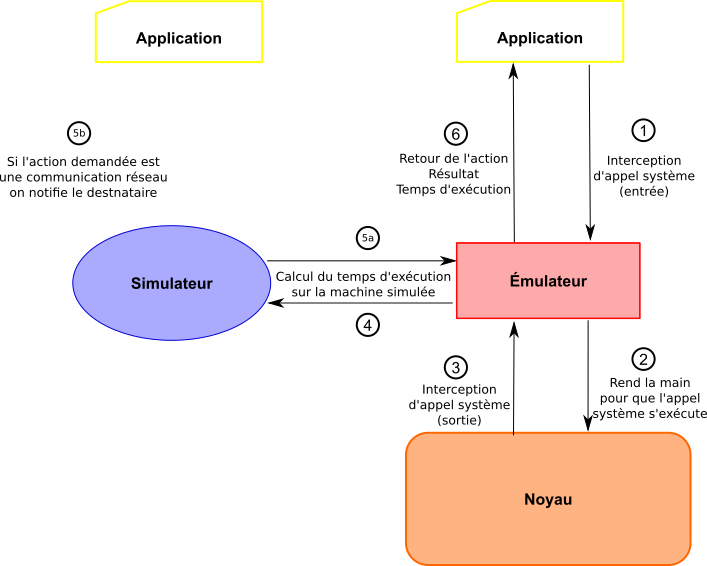
\includegraphics[scale=0.5]{Pictures/png/Emulation_fonctionnement}
   \caption{Fonctionnement de l'émulation par interception.}
   \label{INTERCEPTION}
 \end{figure}
 
Pour intercepter ces actions, il faut d'abord choisir à quel niveau se placer.
En effet, une application peut communiquer avec le noyau via différentes
abstractions. Elle peut soit utiliser les fonctions d'interaction directe avec
le noyau que sont les appels systèmes, soit utiliser les différentes
abstractions fournies par le système d'exploitation: bibliothèques (fonctions de
la libc par exemple) ou les fonctions POSIX dans le cas d'un système UNIX.

\begin{figure}[H]
 \centering
 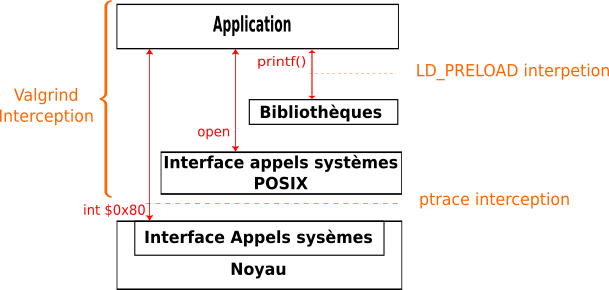
\includegraphics[scale=0.75]{Pictures/png/Communication_application_noyau_v3.png}
 \caption{Communications possibles entre le noyau et une application.}
 \label{AS_Communication}
\end{figure}

Nous allons donc voir comment on peut intercepter et modifier des actions au
niveau de l'application (fichier source puis binaire), des appels systèmes et
des appels de fonctions. Par la suite nous appelerons médiation l'ensemble des
modifications effectuées par l'émulateur sur les actions interceptées.

